\section*{Abstract}
\bigskip

Artificial intelligence is a growing field which aims is to improve task automation. Through this internship, a subfield of artificial intelligence named reinforcement learning has been explored.

Reinforcement learning deals with issues governed by a set of rewards. For example, the classical problem in reinforcement learning is the control of agent through one place to another. The agent receives a reward when it arrives to the final place.  The goal of our control is to find the optimal sequence of actions that maximises the cumulated rewards, which is, for our example, to reach to goal within the shortest time.

THALES is involved in the infrastructure security design, and aims to ensure the security of infrastructures by created plans to scenarios generated by SE-STAR. 
SE-STAR is a simulation capable of created multiple scenarios which may involve a large number of agents. SE-STAR uses internals drives (like hunger, fear, stress ...) to control the mass of agents but these internal drives has to be carefully design to accomplish a scenario (like a fight in a gare).

We choose another way of controlling agents that uses only rewards to automatically find the optimal behaviour that correspond to a given scenario.
Notably, we have worked on the control of an agent in a simulated environnement created by the thales' internal biomimetic simulation SE-STAR.

We will propose various architectures and reinforcement learning algorithms to allow an agent to move in its simulated environnement by its own internal motivations to find our specified goal. The novelty of this approch is to find a policy with a weakly informative input like the partial vision of the agent which banned the use of other traditionnal control algorithms. 

Non-exhaustively, the internship has been divided in five periods:

\begin{itemize}
    \item Bibliographic and litterature search.
    \item Application of main algorithms on simple environnements.
    \item Development of reinforcement learning algorithms on 2D and 3D environnements used by researchers to benchmark their controllers. 
    \item Design of a wrapper around the simulation SE-STAR to support the use of our external algorithm.
    \item Research of algorithms based on intrinsic motivations (or curiosity) to help the agent to find the optimal policy in difficult 3D environnements like those created by SE-STAR. 
\end{itemize} 

\newpage


\section*{Résumé}
\bigskip

L'apprentissage automatique est un domaine subissant actuellement une forte expansion, permettant une automatisation de nombreuses tâches. A travers ce stage, nous avons exploré une sous partie de l'apprentissage automatique qui se nomme l'apprentissage par renforcement profond. 

Ce domaine vise à résoudre des problèmes qui sont régis par des récompenses. Par exemple, nous pouvons imaginer le problème d'un agent ayant pour but d'aller d'un point A à un point B, une récompense serait donnée à l'agent dès qu'il attendra le point B. Notre objectif serait de trouver la politique optimale de l'agent pour maximiser la quantité de récompenses reçues. Dans notre exemple, l'agent aurait à apprendre la séquence d'actions qui permettrait d'aller jusqu'au point B, et ainsi d'obtenir le maximum de récompenses. En particulier, nous travaillerons à l'aide d'un logiciel de simulation bio-inspiré qui se nomme SE-STAR. 

THALES est impliqué dans la conception d'infrastructures critiques. Elle a pour objectif de garantir la sécurité des infrastructures. Pour cela, elle utilise le logiciel SE-STAR qui est une simulation ayant pour but de créer des plans répondant à des scénarios possibles dans l'infrastructure concernée. SE-STAR a la capacité de gérer un grand nombre d'agents simultanément. Pour contrôler ces individus, SE-STAR utilise des motivations (faim, stress, peur ...), néanmoins, pour contrôler une masse d'individus, il faut être précis dans la conception de ces motivations pour accomplir un scénario.

Nous avons choisi une autre voie pour contrôler les agents qui n'utilise que la spécification des récompenses pour générer un comportement correspondant à celui souhaité pour un scénario.
Nous avons donc travaillé sur le contrôle d'un agent dans une simulation crée par SE-STAR.

Nous proposerons une architecture et des algorithmes d'apprentissage par renforcement permettant à un agent de se déplacer dans l'environnement simulé à la recherche de la sortie de façon non supervisée (ou faiblement supervisée). L'intérêt de notre approche est qu'elle utilise des entrées extremment bruitées et partielles (la vision de l'agent) ce qui empêche toutes stratégies de contrôles usuellement appliquées.

De manière non exhaustive, nous pouvons définir ce stage en cinq périodes: 
\begin{itemize}
    \item Découverte et recherche bibliographique.
    \item Application des principaux algorithmes sur des cas simples.
    \item Élaboration d'algorithmes de renforcements profonds sur des environnements 2D et 3D utilisés par les chercheurs pour comparer la performance de leurs méthodes
    \item Conception d'un outil autour de SE-STAR pour supporter les algorithmes d'apprentissage par renforcement.
    \item Recherche autour d'une solution adaptée spécifiquement à l'apprentissage par renforcement profond dans le cadre problématique des environnements labyrinthiques.
\end{itemize}

Ci dessous une représentation des grandes périodes pendant ce stage:

\begin{center}
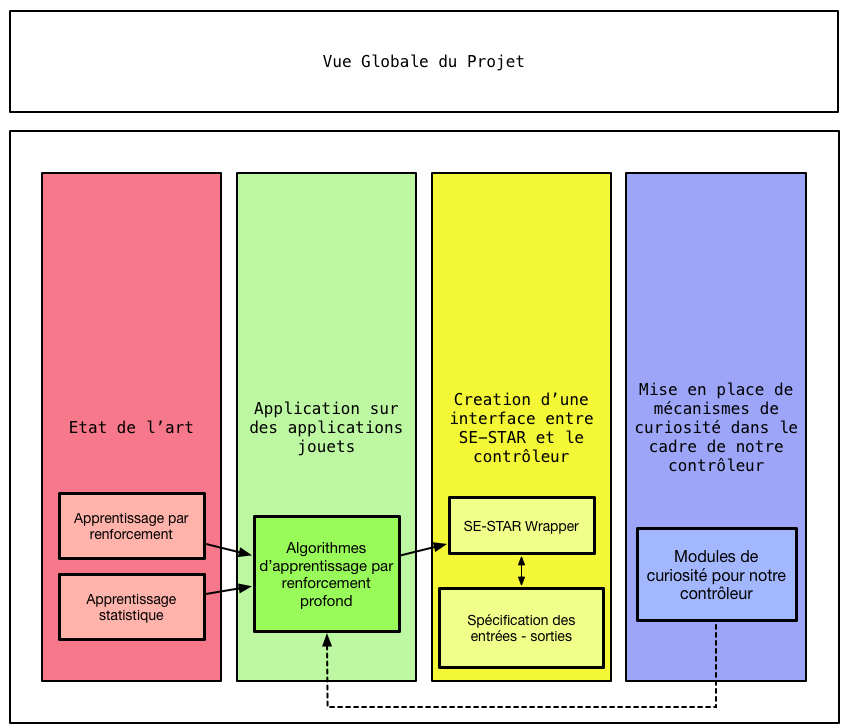
\includegraphics[scale=.5]{./assets/globale.png}
\end{center}
